%!TeX root=../sensetop.tex
\chapter[Chapter \thechapter]{}
\lettrine[lraise=0.3]{T}{heir} intended excursion to Whitwell turned out very different from what Elinor had expected. She was prepared to be wet through, fatigued, and frightened; but the event was still more unfortunate, for they did not go at all.

By ten o'clock the whole party was assembled at the park, where they were to breakfast. The morning was rather favourable, though it had rained all night, as the clouds were then dispersing across the sky, and the sun frequently appeared. They were all in high spirits and good humour, eager to be happy, and determined to submit to the greatest inconveniences and hardships rather than be otherwise.

While they were at breakfast the letters were brought in. Among the rest there was one for Colonel Brandon;—he took it, looked at the direction, changed colour, and immediately left the room.

<What is the matter with Brandon?> said Sir John.

Nobody could tell.

<I hope he has had no bad news,> said Lady Middleton. <It must be something extraordinary that could make Colonel Brandon leave my breakfast table so suddenly.>

In about five minutes he returned.

<No bad news, Colonel, I hope;> said Mrs Jennings, as soon as he entered the room.

<None at all, ma'am, I thank you.>

<Was it from Avignon? I hope it is not to say that your sister is worse.>

<No, ma'am. It came from town, and is merely a letter of business.>

<But how came the hand to discompose you so much, if it was only a letter of business? Come, come, this won't do, Colonel; so let us hear the truth of it.>

<My dear madam,> said Lady Middleton, <recollect what you are saying.>

<Perhaps it is to tell you that your cousin Fanny is married?> said Mrs Jennings, without attending to her daughter's reproof.

<No, indeed, it is not.>

<Well, then, I know who it is from, Colonel. And I hope she is well.>

<Whom do you mean, ma'am?> said he, colouring a little.

<Oh! you know who I mean.>

<I am particularly sorry, ma'am,> said he, addressing Lady Middleton, <that I should receive this letter today, for it is on business which requires my immediate attendance in town.>

<In town!> cried Mrs Jennings. <What can you have to do in town at this time of year?>

<My own loss is great,> he continued, <in being obliged to leave so agreeable a party; but I am the more concerned, as I fear my presence is necessary to gain your admittance at Whitwell.>

What a blow upon them all was this!

<But if you write a note to the housekeeper, Mr Brandon,> said Marianne, eagerly, <will it not be sufficient?>

He shook his head.

<We must go,> said Sir John.—<It shall not be put off when we are so near it. You cannot go to town till tomorrow, Brandon, that is all.>

<I wish it could be so easily settled. But it is not in my power to delay my journey for one day!>

<If you would but let us know what your business is,> said Mrs Jennings, <we might see whether it could be put off or not.>

<You would not be six hours later,> said Willoughby, <if you were to defer your journey till our return.>

<I cannot afford to lose \textit{one} hour.>

Elinor then heard Willoughby say, in a low voice to Marianne, <There are some people who cannot bear a party of pleasure. Brandon is one of them. He was afraid of catching cold I dare say, and invented this trick for getting out of it. I would lay fifty guineas the letter was of his own writing.>

<I have no doubt of it,> replied Marianne.

<There is no persuading you to change your mind, Brandon, I know of old,> said Sir John, <when once you are determined on anything. But, however, I hope you will think better of it. Consider, here are the two Miss Careys come over from Newton, the three Miss Dashwoods walked up from the cottage, and Mr Willoughby got up two hours before his usual time, on purpose to go to Whitwell.>

Colonel Brandon again repeated his sorrow at being the cause of disappointing the party; but at the same time declared it to be unavoidable.

<Well, then, when will you come back again?>

<I hope we shall see you at Barton,> added her ladyship, <as soon as you can conveniently leave town; and we must put off the party to Whitwell till you return.>

<You are very obliging. But it is so uncertain, when I may have it in my power to return, that I dare not engage for it at all.>

<Oh! he must and shall come back,> cried Sir John. <If he is not here by the end of the week, I shall go after him.>

<Ay, so do, Sir John,> cried Mrs Jennings, <and then perhaps you may find out what his business is.>

<I do not want to pry into other men's concerns. I suppose it is something he is ashamed of.>

Colonel Brandon's horses were announced.

<You do not go to town on horseback, do you?> added Sir John.

<No. Only to Honiton. I shall then go post.>

<Well, as you are resolved to go, I wish you a good journey. But you had better change your mind.>

<I assure you it is not in my power.>

He then took leave of the whole party.

<Is there no chance of my seeing you and your sisters in town this winter, Miss Dashwood?>

<I am afraid, none at all.>

<Then I must bid you farewell for a longer time than I should wish to do.>

To Marianne, he merely bowed and said nothing.

<Come Colonel,> said Mrs Jennings, <before you go, do let us know what you are going about.>

He wished her a good morning, and, attended by Sir John, left the room.

The complaints and lamentations which politeness had hitherto restrained, now burst forth universally; and they all agreed again and again how provoking it was to be so disappointed.

<I can guess what his business is, however,> said Mrs Jennings exultingly.

<Can you, ma'am?> said almost every body.

<Yes; it is about Miss Williams, I am sure.>

<And who is Miss Williams?> asked Marianne.

<What! do not you know who Miss Williams is? I am sure you must have heard of her before. She is a relation of the Colonel's, my dear; a very near relation. We will not say how near, for fear of shocking the young ladies.> Then, lowering her voice a little, she said to Elinor, <She is his natural daughter.>

<Indeed!>

<Oh, yes; and as like him as she can stare. I dare say the Colonel will leave her all his fortune.>

When Sir John returned, he joined most heartily in the general regret on so unfortunate an event; concluding however by observing, that as they were all got together, they must do something by way of being happy; and after some consultation it was agreed, that although happiness could only be enjoyed at Whitwell, they might procure a tolerable composure of mind by driving about the country. The carriages were then ordered; Willoughby's was first, and Marianne never looked happier than when she got into it. He drove through the park very fast, and they were soon out of sight; and nothing more of them was seen till their return, which did not happen till after the return of all the rest. They both seemed delighted with their drive; but said only in general terms that they had kept in the lanes, while the others went on the downs.

It was settled that there should be a dance in the evening, and that every body should be extremely merry all day long. Some more of the Careys came to dinner, and they had the pleasure of sitting down nearly twenty to table, which Sir John observed with great contentment. Willoughby took his usual place between the two elder Miss Dashwoods. Mrs Jennings sat on Elinor's right hand; and they had not been long seated, before she leant behind her and Willoughby, and said to Marianne, loud enough for them both to hear, <I have found you out in spite of all your tricks. I know where you spent the morning.>

\begin{figure}[tbph]
\centering
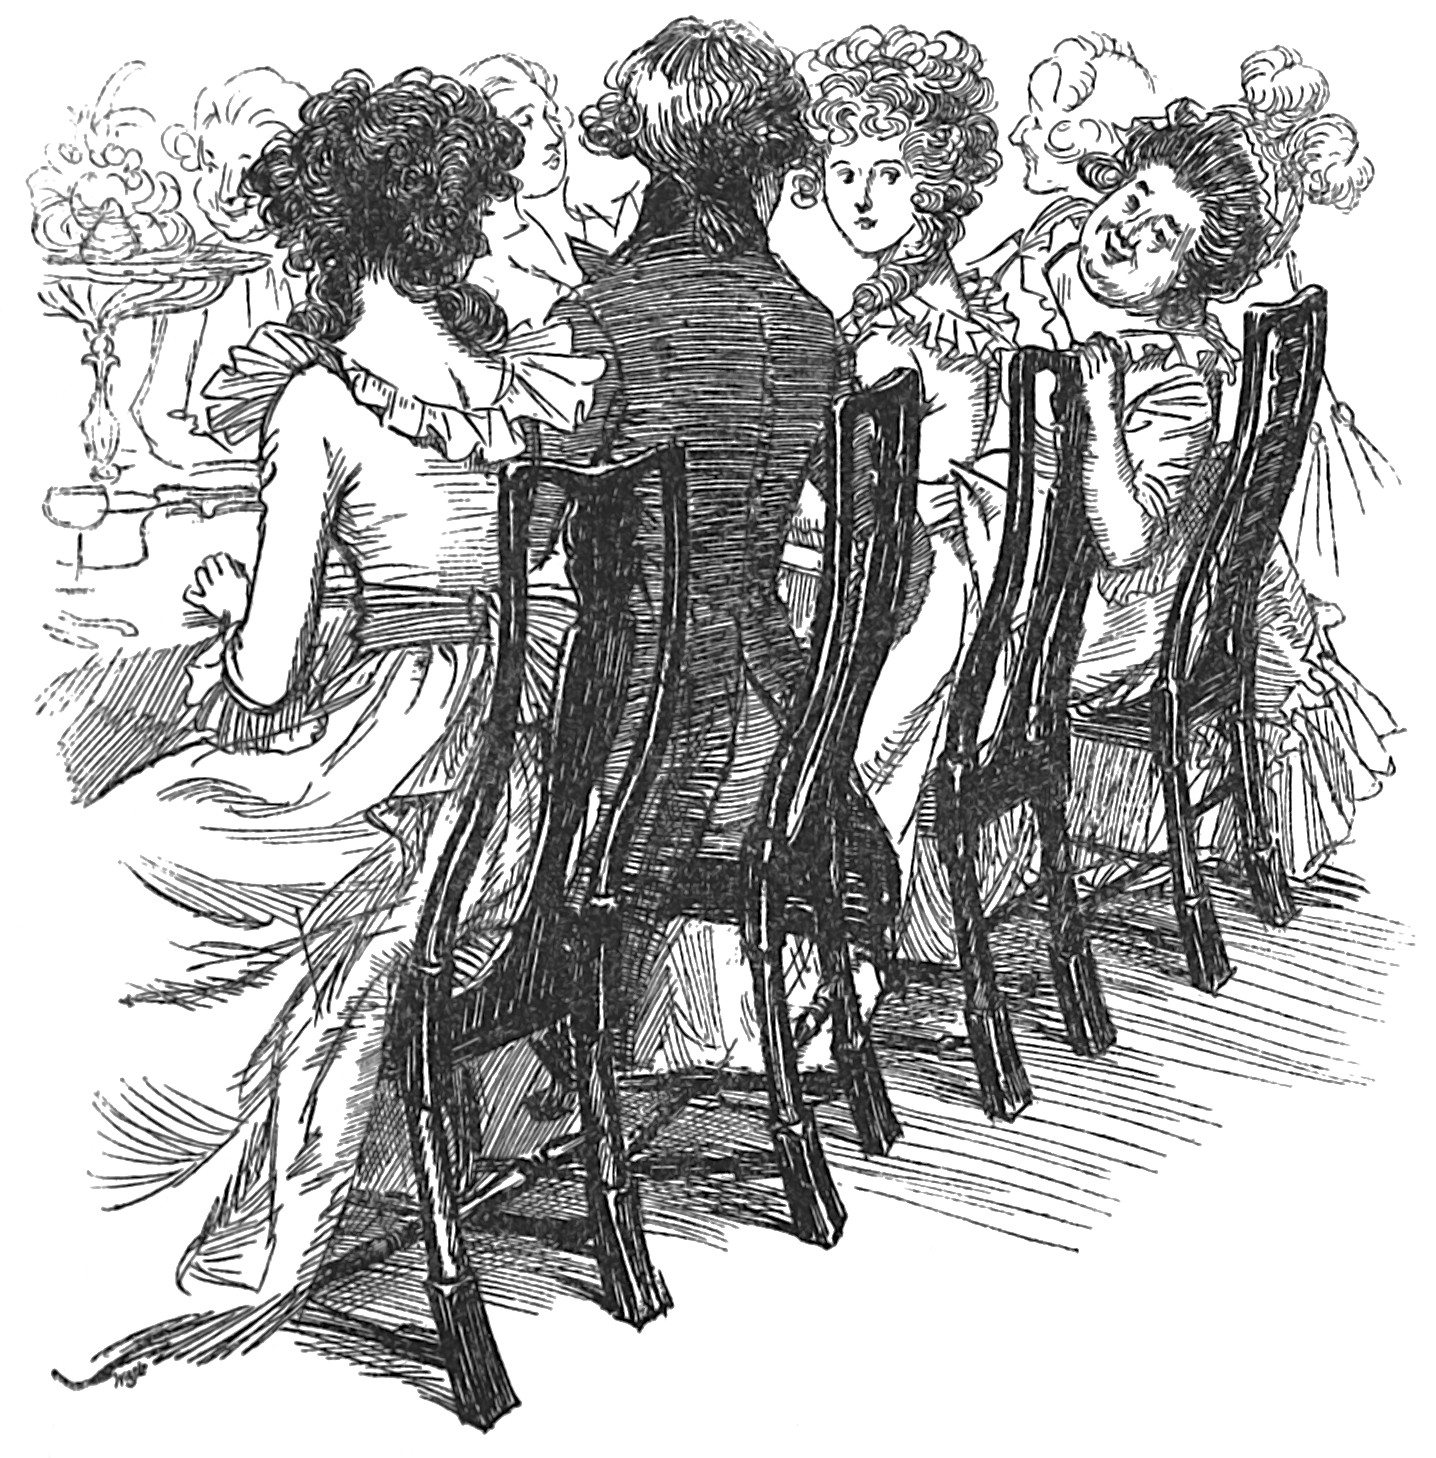
\includegraphics[width=\linewidth]{13tricks}
\caption{<I have found you out in spite of all your tricks.>}
\end{figure}


Marianne coloured, and replied very hastily, <Where, pray?>

<Did not you know,> said Willoughby, <that we had been out in my curricle?>

<Yes, yes, Mr Impudence, I know that very well, and I was determined to find out \textit{where} you had been to. I hope you like your house, Miss Marianne. It is a very large one, I know; and when I come to see you, I hope you will have new-furnished it, for it wanted it very much when I was there six years ago.>

Marianne turned away in great confusion. Mrs Jennings laughed heartily; and Elinor found that in her resolution to know where they had been, she had actually made her own woman enquire of Mr Willoughby's groom; and that she had by that method been informed that they had gone to Allenham, and spent a considerable time there in walking about the garden and going all over the house.

Elinor could hardly believe this to be true, as it seemed very unlikely that Willoughby should propose, or Marianne consent, to enter the house while Mrs Smith was in it, with whom Marianne had not the smallest acquaintance.

As soon as they left the dining-room, Elinor enquired of her about it; and great was her surprise when she found that every circumstance related by Mrs Jennings was perfectly true. Marianne was quite angry with her for doubting it.

<Why should you imagine, Elinor, that we did not go there, or that we did not see the house? Is not it what you have often wished to do yourself?>

<Yes, Marianne, but I would not go while Mrs Smith was there, and with no other companion than Mr Willoughby.>

<Mr Willoughby however is the only person who can have a right to show that house; and as he went in an open carriage, it was impossible to have any other companion. I never spent a pleasanter morning in my life.>

<I am afraid,> replied Elinor, <that the pleasantness of an employment does not always evince its propriety.>

<On the contrary, nothing can be a stronger proof of it, Elinor; for if there had been any real impropriety in what I did, I should have been sensible of it at the time, for we always know when we are acting wrong, and with such a conviction I could have had no pleasure.>

<But, my dear Marianne, as it has already exposed you to some very impertinent remarks, do you not now begin to doubt the discretion of your own conduct?>

<If the impertinent remarks of Mrs Jennings are to be the proof of impropriety in conduct, we are all offending every moment of our lives. I value not her censure any more than I should do her commendation. I am not sensible of having done anything wrong in walking over Mrs Smith's grounds, or in seeing her house. They will one day be Mr Willoughby's, and\longdash>

<If they were one day to be your own, Marianne, you would not be justified in what you have done.>

She blushed at this hint; but it was even visibly gratifying to her; and after a ten minutes' interval of earnest thought, she came to her sister again, and said with great good humour, <Perhaps, Elinor, it \textit{was} rather ill-judged in me to go to Allenham; but Mr Willoughby wanted particularly to show me the place; and it is a charming house, I assure you.—There is one remarkably pretty sitting room up stairs; of a nice comfortable size for constant use, and with modern furniture it would be delightful. It is a corner room, and has windows on two sides. On one side you look across the bowling-green, behind the house, to a beautiful hanging wood, and on the other you have a view of the church and village, and, beyond them, of those fine bold hills that we have so often admired. I did not see it to advantage, for nothing could be more forlorn than the furniture,—but if it were newly fitted up—a couple of hundred pounds, Willoughby says, would make it one of the pleasantest summer-rooms in England.>

Could Elinor have listened to her without interruption from the others, she would have described every room in the house with equal delight.